\subsection{Алгоритм пошуку в ширину}
\label{subsec:bfs-subsection}

Алгоритм пошуку в ширину --- це алгоритм обходу графа, який починається з кореневого вузла і досліджує всі сусідні вузли на поточному рівні глибини, перш ніж перейти на наступний рівень. Це класичний алгоритм, який використовується для обходу графа або деревовидної структури даних.

Алгоритм пошуку в ширину використовує структуру даних у вигляді черги для відстеження вузлів, які потрібно дослідити. Алгоритм починає з додавання кореневого вузла до черги, потім декваліфікує наступний вузол і додає всіх його сусідів до черги. Цей процес продовжується до тих пір, поки не будуть досліджені всі вузли.

Однією з переваг пошуку в ширину є те, що він гарантує найкоротший шлях від кореневої вершини до будь-якої іншої вершини незваженого графа. Це робить його корисним у багатьох додатках, де потрібен найкоротший шлях, наприклад, для пошуку найкоротшого маршруту в дорожній мережі.

Однак пошук в ширину може бути неефективним у графах з великою кількістю ребер, оскільки він повинен дослідити всіх сусідів на кожному рівні, перш ніж перейти на наступний рівень. Це може призвести до додавання великої кількості вузлів до черги, що може спричинити проблеми з пам'яттю.

Таким чином, пошук в ширину - це простий і ефективний алгоритм обходу графа, який корисний у різних додатках, особливо коли потрібно знайти найкоротший шлях. Однак його продуктивність може бути обмежена на великих, складних графах.\\

\begin{figure}[!htp]
    \centering
    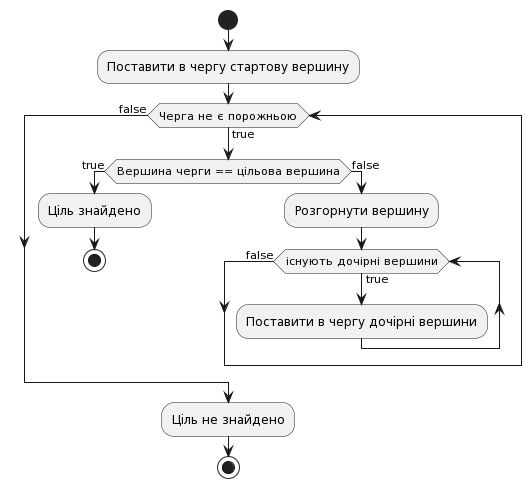
\includegraphics[scale=0.6]{content/chapters/2-implementation-methods/assets/img/bfs_algorithm.png}
    \caption{Блок-схема алгоритму пошуку в ширину}
    \label{fig:bfs}
\end{figure}


Переваги:
\begin{itemize}
    \item Пошук в ширину гарантовано знайде найкоротший шлях до вузла або цілі, якщо вона існує.
    \item Його відносно легко реалізувати і зрозуміти.
    \item Він гарантовано знаходить розв'язок, коли простір пошуку скінченний і коефіцієнт розгалуження скінченний.
    \item Може бути чудовим вибором для додатків, де важливо знайти шлях з найменшою кількістю кроків.
\end{itemize}

Недоліки:
\begin{itemize}
    \item Пошук в ширину може бути повільним і вимагати багато пам'яті, особливо у великих областях пошуку.
    \item Він може витрачати час на дослідження шляхів, які навряд чи приведуть до розв'язку.
    \item Це може бути не найефективніший алгоритм для всіх типів задач, особливо з високим коефіцієнтом розгалуження.
    \item Він може не підходити для задач з нерівномірною вартістю або для задач, де вартість проходження вузла змінюється.
\end{itemize}
